\section{Implementation}
\label{kvdirect:sec:implementation}

Our hardware platform is built on an Intel Stratix V FPGA based programmable NIC (\S\ref{kvdirect:sec:programmable-nic}).
The programmable NIC is attached to the server through two PCIe Gen3 x8 links in a bifurcated x16 physical connector, and contains 4 GiB of on-board DRAM with a single DDR3-1600 channel.

%Predominately, FPGAs are programmed with low-level hardware description languages.
For development efficiency, we use Intel FPGA SDK for OpenCL~\cite{aoc} to synthesize hardware logic from OpenCL.
Our KV processor is implemented in 11K lines of OpenCL code and all kernels are fully pipelined, \ie, the throughput is one operation per clock cycle.
With 180~MHz clock frequency, our design can process KV operations at 180~M op/s if not bottlenecked by network, DRAM or PCIe.

%
%\begin{table}[t!]
%	\centering
%	\caption{Line of code and resource utilization of the KV processor.}
%	\label{kvdirect:tab:resource-util}
%	\scalebox{0.8}{
%		\begin{tabular}{l|r|r|r}
%			\toprule
%			Component & LoC & Logic (\%) & Memory (\%) \\
%			\midrule
%            Hash table & & & \\
%            Slab memory allocator & & & \\
%            Dynamic operation scheduler & & & \\
%            DRAM load dispatcher & & & \\
%            Operation decoder & & & \\
%            \midrule
%            Interconnect & & & \\
%            OpenCL runtime & & & \\
%            Network hard IP & & & \\
%            PCIe DMA and hard IP & & & \\
%            DDR controller & & & \\
%            \midrule
%            Total & & & \\
%			\bottomrule
%		\end{tabular}
%	}
%\end{table}


Below highlights several implementation details.


\begin{figure}[t]
\centering
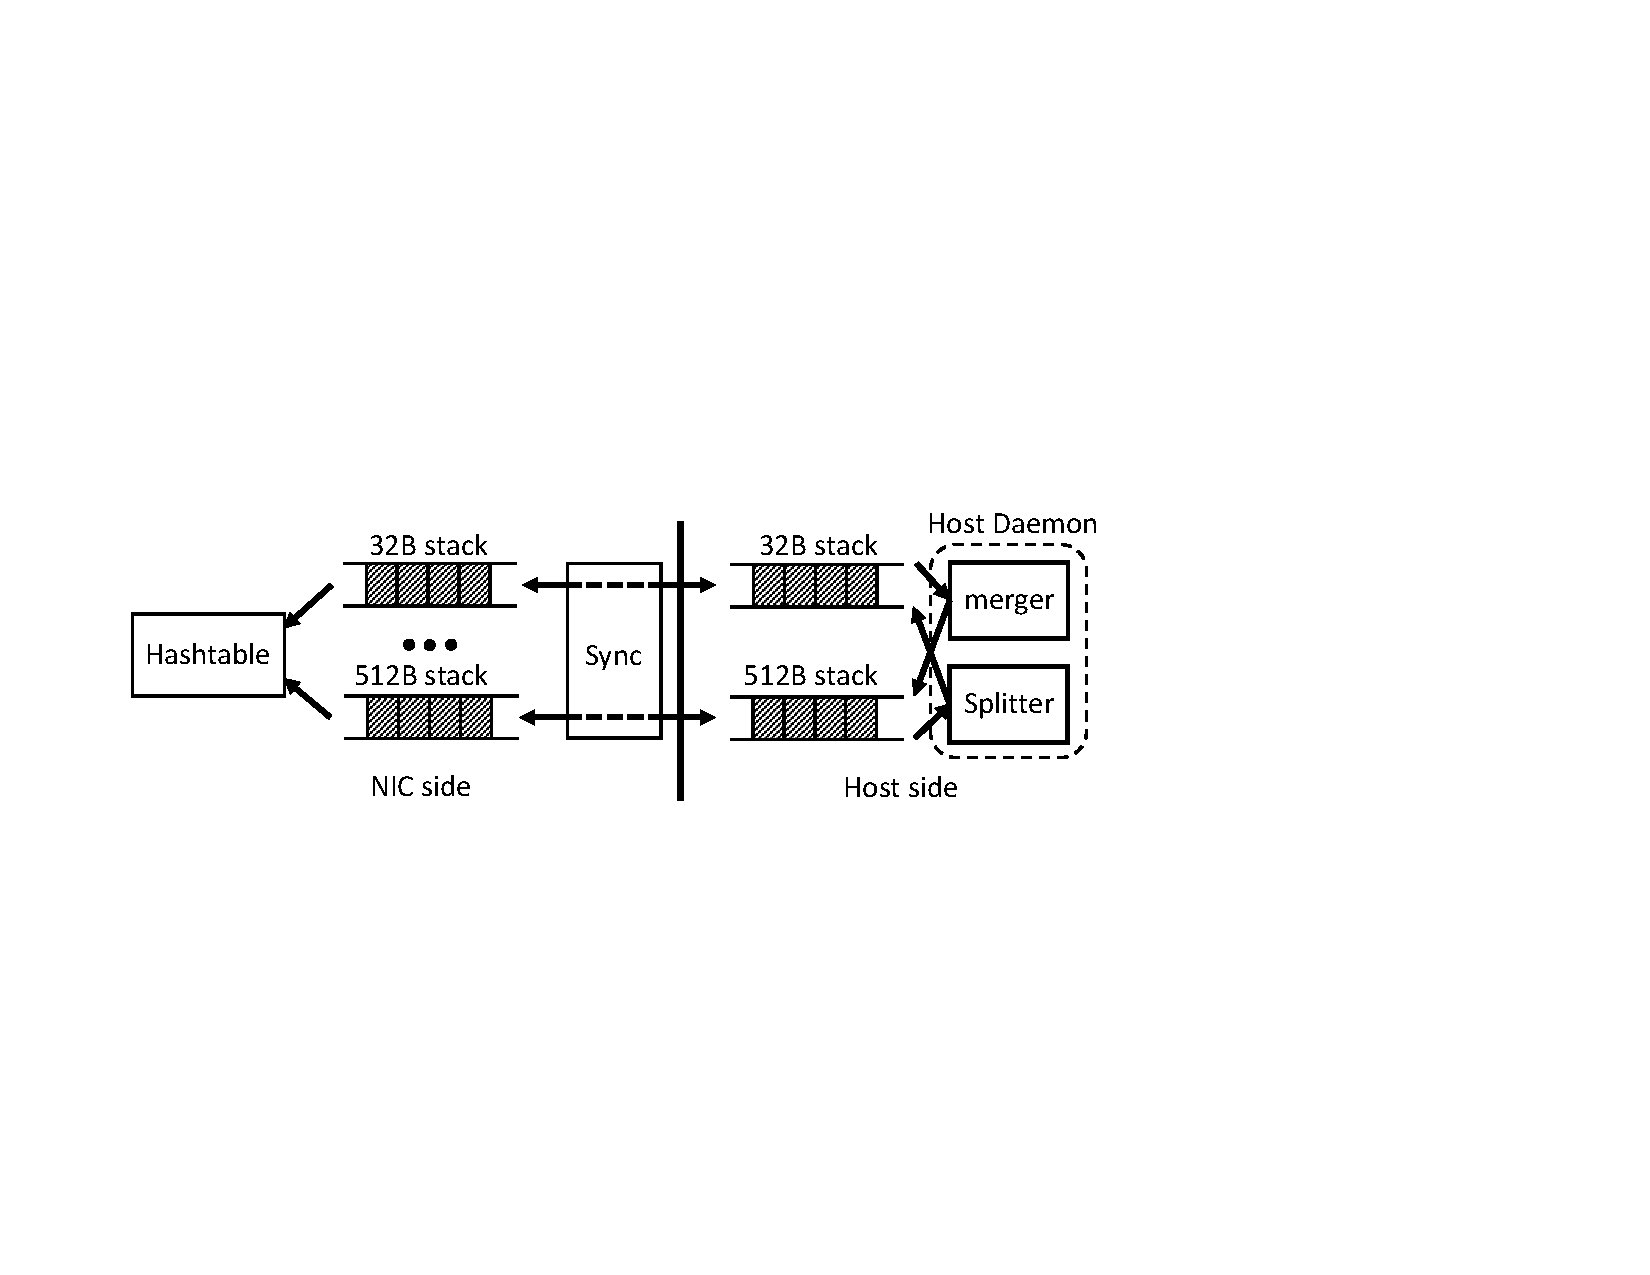
\includegraphics[width=.8\textwidth,page=1]{figure/cropped_slab.pdf}
\caption{Slab memory allocator.}
\label{kvdirect:fig:slab}

\end{figure}


\textbf{Slab Memory Allocator.}
As shown in Figure~\ref{kvdirect:fig:slab}, for each slab size, the slab cache on the NIC is synchronized with host DRAM using two double-ended stacks.
For the NIC-side double-ended stack (left side in Figure~\ref{kvdirect:fig:slab}), the left end is popped and pushed by the allocator and deallocator, and the right end is synchronized with the left end of the corresponding host-side stack via DMA.
The NIC monitors the size of NIC stack and synchronizes to or from the host stack according to high and low watermarks.
Host daemon periodically checks the size of host-side double-ended stack. If it grows above a high watermark, slab merging is triggered; when it drops below a low watermark, slab splitting is triggered.
Because each end of a stack is either accessed by the NIC or the host, and the data is accessed prior to moving pointers, race conditions would not occur.


%In our implementation, each slab entry is 5 bytes and the DMA granularity is 64 bytes, so the amortized DMA overhead per slab operation is $5/64$. Furthermore, when newly freed slab slots are reused by subsequent allocations, the on-NIC stack is used instead of DMA.


%\textbf{Dynamic Operation Scheduler.}
%Upon simultaneous completion of an operation and arrival of a new operation, the reservation station prioritizes completion processing, because the completed operation has waited longer and prioritizing it benefits tail latency.
%During checking and execution of a hash slot, new completions may come.
%For simplicity, we finish scanning the chain of pending operations before moving to another key.

\textbf{DRAM Load Dispatcher.}
One technical challenge is the storage of metadata in DRAM cache, which requires additional 4 address bits and one dirty flag per 64-byte cache line.
Cache valid bit is not needed because all KVS storage is accessed exclusively by the NIC.
To store the 5 metadata bits per cache line, extending the cache line to 65 bytes would reduce DRAM performance due to unaligned access; saving the metadata elsewhere will double memory accesses.
Instead, we leverage spare bits in ECC DRAM for metadata storage.
ECC DRAM typically has 8 ECC bits per 64 bits of data.
For Hamming code to correct one bit of error in 64 bits of data, only 7 additional bits are required.
The 8th ECC bit is a parity bit for detecting double-bit errors.
As we access DRAM in 64-byte granularity and alignment, there are 8 parity bits per 64B data.
We increase the parity checking granularity from 64 data bits to 256 data bits, so double-bit errors can still be detected. This allows us to have 6 extra bits which can save our address bits and dirty flag.

%\textbf{KV Operation Decoder.}
%The KV operation decoder saves receive timestamp and UDP flow tuple as execution context in reservation station.
%When the KV operation completes, the flow control component measures the processing delay from the receive timestamp in execution context.
%The network encoder needs the flow tuple to generate completion packets and send to the client.
%To avoid head-of-line blocking, KV operations are processed out-of-order, so the client may receive KV completions in a different order from requests.
%The client could match the completions with requests by the key, because completions with a same key are guaranteed to be in request order.

\textbf{Vector Operation Decoder.}
%Throughout the KV processor design, we see batching as an universal principle in fetching multiple hash slots in one bucket, synchronizing free slab queues with host memory, lazy splitting and merging of slab slots, and data forwarding of dependent KV operations.
%Batching improves performance by amortizing control plane overhead to multiple data plane payloads.
Compared with PCIe, network is a more scarce resource with lower bandwidth (5~GB/s) and higher latency (2~$\mu$s).
%The control plane overhead of network is also larger. 
An RDMA write packet over Ethernet has 88 bytes of header and padding overhead, while a PCIe TLP packet has only 26 bytes of overhead.
This is why previous FPGA-based key-value stores~\cite{blott13hotcloud,blott2015scaling} have not saturated the PCIe bandwidth, although their hash table designs are less efficient than KV-Direct.
This calls for \textit{client-side batching} in two aspects: batching multiple KV operations in one packet and supporting vector operations for a more compact representation. Towards this end, we implement a decoder in the KV-engine to unpack multiple KV operations from a single RDMA packet.
%For computation efficiency, we could not use a general-purpose compression algorithm.
Observing that many KVs have a same size or repetitive values, the KV format includes two flag bits to allow copying key and value size, or the value of the previous KV in the packet.
%For atomic and vector operations, additional fields include the opcode of the $\lambda$ function and the parameter to the active message.
Fortunately, many significant workloads (\textit{e.g.} graph traversal, parameter server) can issue KV operations in batches.
Looking forward, batching would be unnecessary if higher-bandwidth network is available.
